\documentclass{article}
%\usepackage[superscript]{cite}
\usepackage[pdftex]{graphicx}
\usepackage{sidecap}
\usepackage{caption}
\usepackage{subcaption}
\usepackage{amsmath}
\usepackage{amsfonts}
\usepackage{tikz}
\usepackage{pgfplots}
\usepackage[colorlinks=true,linkcolor=blue,citecolor=blue]{hyperref}
\usepackage{fullpage}
%\usepackage{natbib}
\usepackage[utf8]{inputenc}
\usepackage[english]{babel}
\newcommand{\angstrom}{\text{\normalfont\AA}}
\usepackage[T1]{fontenc}

\begin{document}
%\section{Phase I}
%We want to define the scope of the current project such that it is something we feel we can accomplish, and be relatively complete in our data collection.
%


\section{Procedure}
%Three primary tasks 
%\begin{itemize}
%\item \textbf{Data Research} The person assigned to data research will search the literature to find out \underline{what data has been taken for a given nova.} 
%\item \textbf{Data Acquisition} The person assigned to retrieving the data: this can mean either downloading the data or contacting the author of the original paper.
%\item \textbf{Data Importation} The person assigned to incorporating the data into the ONC software.
%\end{itemize}
Three step procedure:
\begin{itemize}
\item \textbf{Data Research} Data research involves searching the literature to find out what data has been taken for a given nova.
\item \textbf{Data Acquisition} Retrieving the data. This can mean either downloading the data or contacting the author of the original paper.
\item \textbf{Data Importation} Incorporating the data into the ONC software.
\end{itemize}


\section{Ticket System}
We will use the ticket system: each new piece of data will be assigned a ticket. This serves a two-fold purpose: 
\begin{enumerate}
\item  It ensures that we are, at the very least, aware of all of the data that has been used in published articles for a given nova.
\item It ensures that, from the start, we maintain an accurate provenance for each piece of data, as well as complete meta-data.
\end{enumerate}

Tickets will be initially created in the data research step, and fields will be filled in during both the data research and data acquisition steps. A complete ticket means that the data is ready to be incorporated into the ONC.

\subsection{When to Make a New Ticket}
There are several factors that determine when a new ticket should be generated
\begin{enumerate}
\item \textbf{Reference} A single ticket should never have multiple references. If the same group took data on the same nova, using the same telescope/instrument, but published part of it in a different article, it will still get its own ticket.
\item \textbf{Nova} If a single reference has data for multiple novae, every novae from that reference will get its own ticket. 
\item \textbf{Data Types} If a single paper publishes both photometry and spectra, each of these should get their own ticket. This is because the meta-data associated with photometry and spectra are different. 
\item \textbf{Wavelength Regime} If a single paper publishes both radio and optical photometry, each of these should get their own ticket. This is done mostly for the ease of bookkeeping.
\end{enumerate}


\subsection{When NOT to Make a New Ticket}
There are also several cases that may seem like they would necessitate different tickets but do not.
\begin{enumerate}
\item \textbf{Telescopes/Observers/Filter Systems} Most collection of spectra and photometry are a compilation from many different telescopes, observers, and filter systems (e.g. AAVSO). Giving each one their own ticket would end up generating a flood of tickets for each data collection. So, instead, we have included the ability to specify different Telescopes/Observers/Filter Systems in the data file, by allowing the user to specify columns within the file that provide information on these differences.
\end{enumerate}

%There are two factors that determine 

\subsection{Naming Convention}
To make parsing/understanding individual tickets easier, we will use a specific naming convention for them. Every ticket should use the following naming convention:\\

\noindent
\begin{Large}
$<$\texttt{Nova Name}$>$\_$<$\texttt{First Author}$>$\_$<$\texttt{Wavelength Regime}$>$\_$<$\texttt{Data Type}$>$.txt
\end{Large}
\\
Where data type can be photometry, spectra, or image.

So, for instance, if the ticket was for the radio photometry for FH Ser taken from Hjellming et al. (1979) the ticket name would be:
\\

\noindent
\begin{Large}
FHSer\_Hjellming\_Radio\_Photometry.txt
\end{Large}


\subsection{Photometry Tickets}
An example of a photometry ticket can be found in Section~\ref{sec:ExampTickPhot}. More details will come in the next update to the procedure section. 


\subsection{Spectra Tickets}
The primary difference between the spectra tickets and the photometry tickets is that there's a good chance that you'll have multiple spectra in a single ticket. It is relatively common for a single paper to have spectra from multiple telescopes/instruments, each of which can/will have varying resolution and SNR.

Rather than generating multiple tickets for all of these spectra, we will instead have a single ticket that points to a separate meta data file that is \emph{comma delimited}, with columns that provide requisite meta data for each spectra that you pull from a single reference/article. 

This means that the primary purpose of the ticket will be to serve as a pointer to the secondary meta data file, detailing what every column of this secondary meta data file holds. An example of a spectra ticket can be found in section~\ref{sec:ExampTickSpectra}; an example of the spectra meta data file can be found in section~\ref{sec:ExampTickSpectraMetaDataFile}. 

\textbf{NOTE:} Feel free to write the spectra meta data file in Excel or the open office equivalent; just remember that you \emph{must save it as a csv file.}









\section{Data Research}
\subsection{Finding Novae}
Before you can start looking for data on novae you need to actually know what novae exist. \textbf{NOTE} At this beginning stage we will only be working on novae that have gone off in the Milky Way (galactic novae). A thorough list of galactic novae can be found here \url{http://projectpluto.com/galnovae/galnovae.txt}. 

\subsubsection{Naming Convention for Novae}
When a nova is first observed there is usually a period of time where it isn't entirely clear that it is in fact a nova. From an observers perspective, it just looks like a new bright thing in the sky. It needs to be confirmed as a nova, something that is usually done spectroscopically.

However, when all you have is just a new bright thing (and you think it might be a nova) people will refer to it as PNV J17574766+0444243: PNV means "possible nova", and the rest of the name is its specific coordinates (RA=17:57:47.66, Dec=+04:44:23.3).

Once the new bright thing has been confirmed to be a nova it still needs an "official" name, which usually takes time. While waiting for the "official" name, most astronomers use a shorthand name to describe it. The convention for this shorthand is:\\

\noindent
%\begin{Large}
\textbf{Nova (or just N)} $<$\texttt{Constellation the nova was found in}$>$ $<$\texttt{Year the nova was found in}$>$ 
%\end{Large}
So, if there is a nova found in the constellation Sagittarius in 2015, then the name of the nova would be \textbf{Nova Sgr 2015} (Sgr is the shorthand for Sagittarius). If there were more than one nova in a given year in Sagittarius, then you would have to append a number 2 at the end. So the second nova in Sgr would be \textbf{Nova Sgr 2015 2}. 

The nova will finally get an "official" name that is based on what number event this was in the particular constellation, usually prepended with the letter V. So, for instance, for the above nova, it was given the name V5667 Sgr. 

To make a long story short, there is a good chance that you will run into multiple names for the same nova. To check what different names exist for a single nova you can go to VSX Search (\url{https://www.aavso.org/vsx/index.php?view=search.top}).





\subsection{Finding Papers/Literature}
Your primary resource for data research will be ads (\url{http://adsabs.harvard.edu/abstract_service.html}). This allows you to search by author, title keywords, abstract keywords, etc.

More details will come in the next update to the procedure section. 









\newpage
\appendix
\section{Example: Ticket for FH Ser Radio (Photometry) Data}
\label{sec:ExampTickPhot}
\begin{itemize}
\item \textbf{OBJECT NAME:} FHSer
\item \textbf{TIME UNITS:} Days
\item \textbf{FLUX UNITS:} mJy
\item \textbf{FLUX ERROR UNITS:} mJy
\item \textbf{FILTER SYSTEM:} NA
\item \textbf{MAGNITUDE SYSTEM:} NA
\item \textbf{WAVELENGTH REGIME:} Radio
\item \textbf{TIME SYSTEM:} MJD
\item \textbf{ASSUMED DATE OF OUTBURST:}
%\item \textbf{UPPER LIMIT:} 
\item \textbf{TELESCOPE:} NA
\item \textbf{INSTRUMENT:} NA
%\item \textbf{OBSERVATORY:} VLA
\item \textbf{OBSERVER:} Hjellming, R.
\item \textbf{REFERENCE:} 1979AJ.....84.1619H
\item \textbf{DATA FILENAME:}
\item \textbf{TIME COLUMN NUMBER:}
\item \textbf{FLUX COLUMN NUMBER:} 
\item \textbf{FLUX ERROR COLUMN NUMBER:} 
%\item \textbf{FILTER \emph{or} FREQUENCY \emph{or} ENERGY RANGE COLUMN NUMBER:} 
\item \textbf{FILTER/FREQUENCY/ENERGY RANGE COLUMN NUMBER:} 
\item \textbf{UPPER LIMIT FLAG COLUMN NUMBER:} 
\item \textbf{TELESCOPE COLUMN:} NA
\item \textbf{INSTRUMENT COLUMN:} NA
\item \textbf{OBSERVER COLUMN:} NA
\item \textbf{TICKET STATUS:} Waiting for acquisition.
\end{itemize}






\newpage
\section{Example: Ticket for V1324 Sco Optical Spectra Data}
\label{sec:ExampTickSpectra}
\begin{itemize}
\item \textbf{OBJECT NAME:} V1324Sco
\item \textbf{WAVELENGTH REGIME:} Optical
\item \textbf{TIME SYSTEM:} MJD
\item \textbf{ASSUMED DATE OF OUTBURST:} NA
\item \textbf{REFERENCE:} Finzell et al (In Prep)
\item \textbf{METADATA FILENAME:} Optical/Spectra/Finzell/ V1324Sco\char`_Finzell\char`_Optical\char`_Spectra\char`_METADataFile.csv
\item \textbf{FILENAME COLUMN:} 0
\item \textbf{WAVELENGTH COLUMN NUMBER:} 1
\item \textbf{FLUX COLUMN NUMBER:} 2
\item \textbf{FLUX ERROR COLUMN NUMBER:} 3
\item \textbf{FLUX UNITS COLUMN:} 5
\item \textbf{DATE COLUMN:} 6
\item \textbf{TELESCOPE COLUMN:} 8
\item \textbf{INSTRUMENT COLUMN:} 9
\item \textbf{OBSERVER COLUMN:} 7
\item \textbf{SNR COLUMN:} NA
\item \textbf{DISPERSION COLUMN:} 9
\item \textbf{WAVELENGTH RANGE COLUMN:}10,11
\item \textbf{DEREDDENED FLAG:} False
\item \textbf{TICKET STATUS:} COMPLETED
\end{itemize}

\subsection{Example: Meta Data File for V1324 Sco Optical Spectra Data}
\label{sec:ExampTickSpectraMetaDataFile}
\begin{figure}[h]
\centering
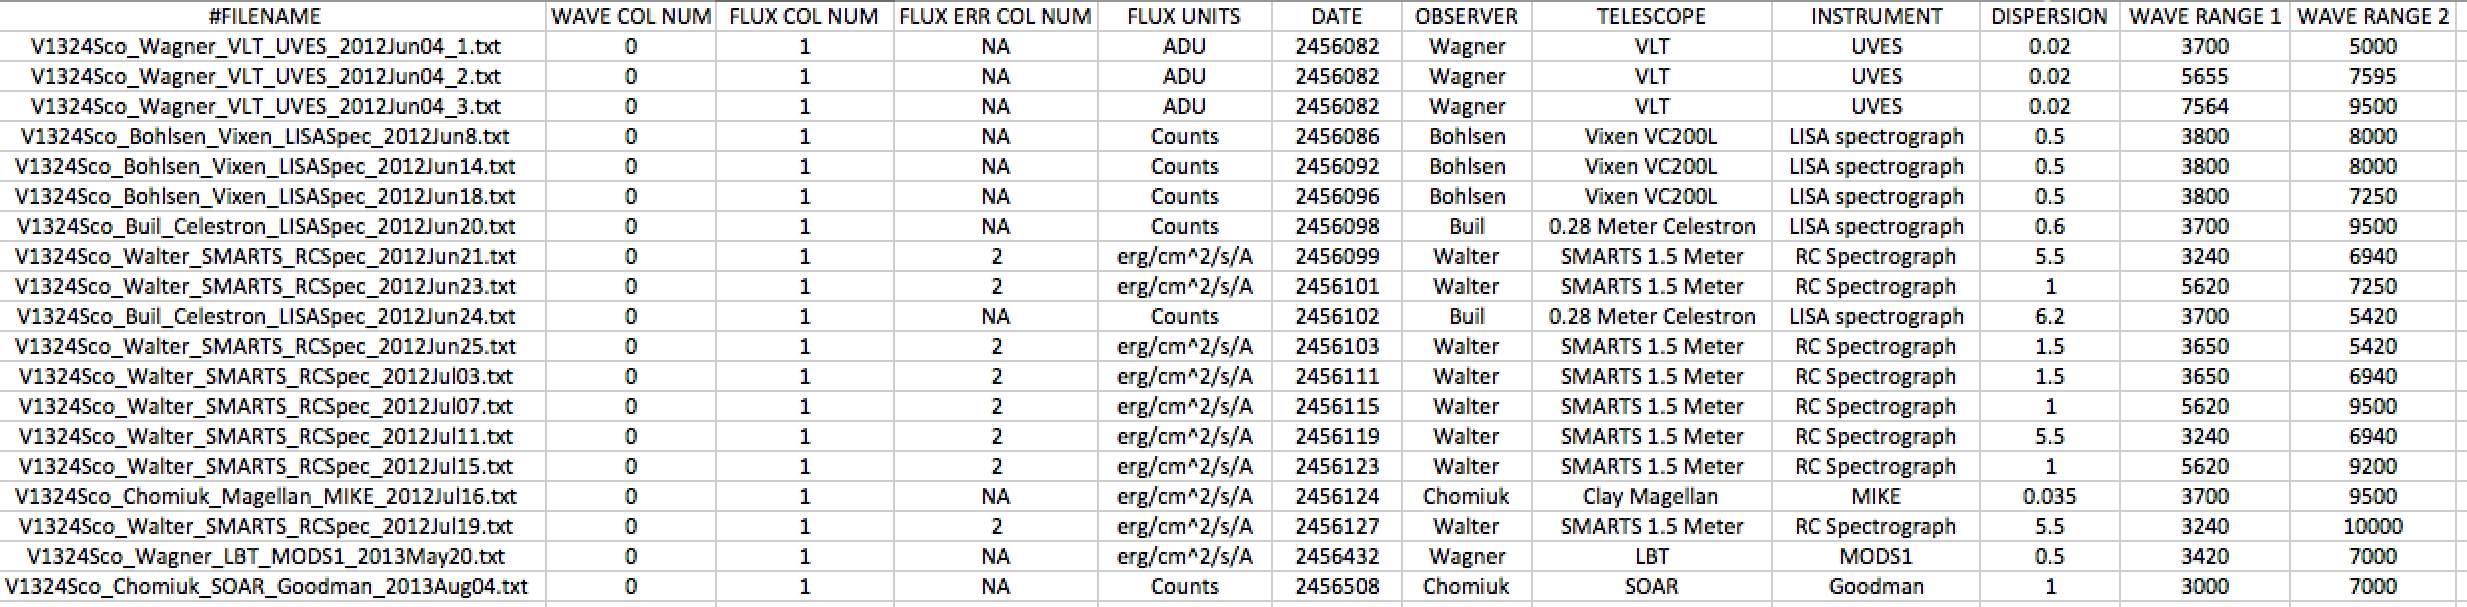
\includegraphics[width=15cm]{Spectra_MetaDataFile_Example} 
%\caption{ }
%\label{fig:1}
\end{figure}






%Hopefully we will be able to implement multiple phases of 


%
%\section*{Guiding Principles}
%These are taken from James' paper. Since we are already using James' format, some of the principles are (essentially) built in for us, so I've reordered them based on what I think will be most important for us to keep in mind as we move along.
%
%\begin{itemize}
%\item \textbf{Accuracy and Accountability}: We need to make sure that we include \emph{all} relevant information for any given dataset
%\item \textbf{Completeness and Persistence}: We need to hunt down all possible data sources with a fervent determination. Our goal should always be to have \emph{everything that is publicly available}. There is no such thing as a dataset too small.
%\item \textbf{Community Driven}: The more we can get people involved and invested, the easier our job will be.
%\item \textbf{Accessibility}
%\item \textbf{Integration}
%
%\end{itemize}
%
%
%
%\section*{Tasks}
%\begin{itemize}
%\item \textbf{Data Collection}: This will be an ongoing process, and falls under the purview of the data acquisition leader. Here is a list of tasks that we can do to get started.
%\begin{enumerate}
%\item Contact Fred Walter and Ulisse Munari, who already have extensive datasets for southern and northern novae, respectively.  
%\item Pull from AAVSO. I believe we can do this in an automated way.
%\item Get radio data, both from e-NOVA and from literature.
%\end{enumerate}
%\item \textbf{Data Formatting}: This falls under the purview of the software leader
%\begin{enumerate}
%\item Determine what format James' software is going to be expecting 
%\item Write software that will reformat the data so that it is compatible with James' software. 
%\end{enumerate}
%\item \textbf{Quality Control}: This falls under the purview of the quality control leader
%\begin{enumerate}
%\item Make sure that all data can be traced back to its origin
%\item Make sure that all measured values have associated uncertainties. I'm not sure what we should do with data that doesn't have uncertainties...
%\end{enumerate}
%\end{itemize}
%
%
%
%%\section{Specific Leader Roles}
%%\begin{itemize}
%%\textbf{Data Collection}
%%\textbf{Software Design}
%%\textbf{Quality Control}
%%\end{itemize}
%
%%This isn't to say that the entire burden will be on
%
%
%
%
%
%





\end{document}